\documentclass[crop,tikz]{standalone} 
\usepackage{tikz, amsmath, amssymb, graphicx} 

\DeclareMathAlphabet\mathbfcal{OMS}{cmsy}{b}{n}

\newcommand{\Mt}{\mathbfcal{M}}
\newcommand{\Yt}{\mathbfcal{Y}}
\newcommand{\Ft}{\mathbfcal{F}}

\usetikzlibrary{positioning, shapes.geometric} 
\usetikzlibrary{backgrounds}

\begin{document} 

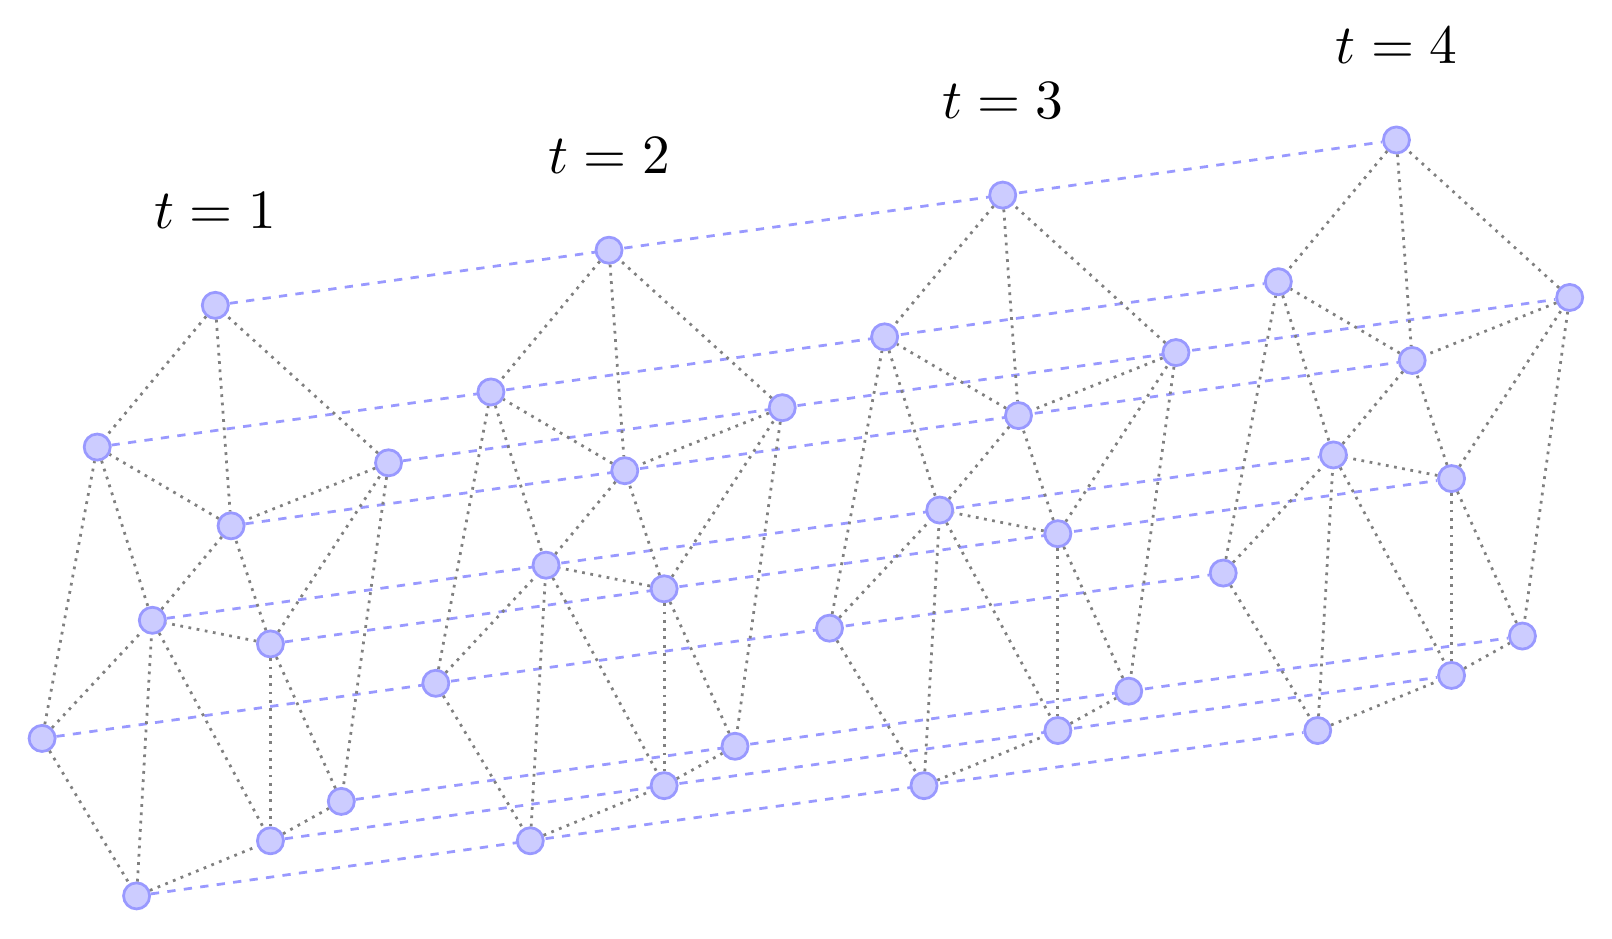
\begin{tikzpicture} 


\tikzstyle{node_style} = [circle,draw=blue!40!,fill=blue!20!, line width=1]

\tikzstyle{edge_style} = [draw=gray, line width=1, dotted]

\tikzstyle{edge_style2} = [draw=blue!40!, line width=1, dashed]


\node[inner sep=0pt, scale=2] at (3, 10) {$t=1$};
\node[inner sep=0pt, scale=2] at (8, 10.7) {$t=2$};
\node[inner sep=0pt, scale=2] at (13, 11.4) {$t=3$};
\node[inner sep=0pt, scale=2] at (18, 12.1) {$t=4$};

\node[node_style] (v0) at (3.70, 4.50) {};
\node[node_style] (v1) at (5.20, 6.80) {};
\node[node_style] (v2) at (0.80, 3.30) {};
\node[node_style] (v3) at (3.00, 8.80) {};
\node[node_style] (v4) at (2.00, 1.30) {};
\node[node_style] (v5) at (1.50, 7.00) {};
\node[node_style] (v6) at (2.20, 4.80) {};
\node[node_style] (v7) at (3.20, 6.00) {};
\node[node_style] (v8) at (3.70, 2.00) {};
\node[node_style] (v9) at (4.60, 2.50) {};
\node[node_style] (v10) at (8.70, 5.20) {};
\node[node_style] (v11) at (10.20, 7.50) {};
\node[node_style] (v12) at (5.80, 4.00) {};
\node[node_style] (v13) at (8.00, 9.50) {};
\node[node_style] (v14) at (7.00, 2.00) {};
\node[node_style] (v15) at (6.50, 7.70) {};
\node[node_style] (v16) at (7.20, 5.50) {};
\node[node_style] (v17) at (8.20, 6.70) {};
\node[node_style] (v18) at (8.70, 2.70) {};
\node[node_style] (v19) at (9.60, 3.20) {};
\node[node_style] (v20) at (13.70, 5.90) {};
\node[node_style] (v21) at (15.20, 8.20) {};
\node[node_style] (v22) at (10.80, 4.70) {};
\node[node_style] (v23) at (13.00, 10.20) {};
\node[node_style] (v24) at (12.00, 2.70) {};
\node[node_style] (v25) at (11.50, 8.40) {};
\node[node_style] (v26) at (12.20, 6.20) {};
\node[node_style] (v27) at (13.20, 7.40) {};
\node[node_style] (v28) at (13.70, 3.40) {};
\node[node_style] (v29) at (14.60, 3.90) {};
\node[node_style] (v30) at (18.70, 6.60) {};
\node[node_style] (v31) at (20.20, 8.90) {};
\node[node_style] (v32) at (15.80, 5.40) {};
\node[node_style] (v33) at (18.00, 10.90) {};
\node[node_style] (v34) at (17.00, 3.40) {};
\node[node_style] (v35) at (16.50, 9.10) {};
\node[node_style] (v36) at (17.20, 6.90) {};
\node[node_style] (v37) at (18.20, 8.10) {};
\node[node_style] (v38) at (18.70, 4.10) {};
\node[node_style] (v39) at (19.60, 4.60) {};


\begin{scope}[on background layer]
\draw[edge_style2]  (v0) edge (v30);
\draw[edge_style2]  (v1) edge (v31);
\draw[edge_style2]  (v2) edge (v32);
\draw[edge_style2]  (v3) edge (v33);
\draw[edge_style2]  (v4) edge (v34);
\draw[edge_style2]  (v5) edge (v35);
\draw[edge_style2]  (v6) edge (v36);
\draw[edge_style2]  (v7) edge (v37);
\draw[edge_style2]  (v8) edge (v38);
\draw[edge_style2]  (v9) edge (v39);
\end{scope}



\draw[edge_style]  (v0) edge (v9);
\draw[edge_style]  (v0) edge (v8);
\draw[edge_style]  (v0) edge (v7);
\draw[edge_style]  (v0) edge (v6);
\draw[edge_style]  (v0) edge (v1);
\draw[edge_style]  (v1) edge (v9);
\draw[edge_style]  (v1) edge (v7);
\draw[edge_style]  (v1) edge (v3);
\draw[edge_style]  (v3) edge (v7);
\draw[edge_style]  (v3) edge (v5);
\draw[edge_style]  (v6) edge (v7);
\draw[edge_style]  (v5) edge (v6);
\draw[edge_style]  (v6) edge (v8);
\draw[edge_style]  (v2) edge (v5);
\draw[edge_style]  (v2) edge (v6);
\draw[edge_style]  (v2) edge (v4);
\draw[edge_style]  (v4) edge (v6);
\draw[edge_style]  (v4) edge (v8);
\draw[edge_style]  (v8) edge (v9);
\draw[edge_style]  (v7) edge (v5);

\draw[edge_style]  (v10) edge (v19);
\draw[edge_style]  (v10) edge (v18);
\draw[edge_style]  (v10) edge (v17);
\draw[edge_style]  (v10) edge (v16);
\draw[edge_style]  (v10) edge (v11);
\draw[edge_style]  (v11) edge (v19);
\draw[edge_style]  (v11) edge (v17);
\draw[edge_style]  (v11) edge (v13);
\draw[edge_style]  (v13) edge (v17);
\draw[edge_style]  (v13) edge (v15);
\draw[edge_style]  (v16) edge (v17);
\draw[edge_style]  (v15) edge (v16);
\draw[edge_style]  (v16) edge (v18);
\draw[edge_style]  (v12) edge (v15);
\draw[edge_style]  (v12) edge (v16);
\draw[edge_style]  (v12) edge (v14);
\draw[edge_style]  (v14) edge (v16);
\draw[edge_style]  (v14) edge (v18);
\draw[edge_style]  (v18) edge (v19);
\draw[edge_style]  (v17) edge (v15);

\draw[edge_style]  (v20) edge (v29);
\draw[edge_style]  (v20) edge (v28);
\draw[edge_style]  (v20) edge (v27);
\draw[edge_style]  (v20) edge (v26);
\draw[edge_style]  (v20) edge (v21);
\draw[edge_style]  (v21) edge (v29);
\draw[edge_style]  (v21) edge (v27);
\draw[edge_style]  (v21) edge (v23);
\draw[edge_style]  (v23) edge (v27);
\draw[edge_style]  (v23) edge (v25);
\draw[edge_style]  (v26) edge (v27);
\draw[edge_style]  (v25) edge (v26);
\draw[edge_style]  (v26) edge (v28);
\draw[edge_style]  (v22) edge (v25);
\draw[edge_style]  (v22) edge (v26);
\draw[edge_style]  (v22) edge (v24);
\draw[edge_style]  (v24) edge (v26);
\draw[edge_style]  (v24) edge (v28);
\draw[edge_style]  (v28) edge (v29);
\draw[edge_style]  (v27) edge (v25);

\draw[edge_style]  (v30) edge (v39);
\draw[edge_style]  (v30) edge (v38);
\draw[edge_style]  (v30) edge (v37);
\draw[edge_style]  (v30) edge (v36);
\draw[edge_style]  (v30) edge (v31);
\draw[edge_style]  (v31) edge (v39);
\draw[edge_style]  (v31) edge (v37);
\draw[edge_style]  (v31) edge (v33);
\draw[edge_style]  (v33) edge (v37);
\draw[edge_style]  (v33) edge (v35);
\draw[edge_style]  (v36) edge (v37);
\draw[edge_style]  (v35) edge (v36);
\draw[edge_style]  (v36) edge (v38);
\draw[edge_style]  (v32) edge (v35);
\draw[edge_style]  (v32) edge (v36);
\draw[edge_style]  (v32) edge (v34);
\draw[edge_style]  (v34) edge (v36);
\draw[edge_style]  (v34) edge (v38);
\draw[edge_style]  (v38) edge (v39);
\draw[edge_style]  (v37) edge (v35);




\end{tikzpicture}
\end{document} 
